\documentclass[12pt]{article}

\usepackage{amsmath}
\usepackage{amssymb}
\usepackage{amsfonts}
\usepackage[style=iso]{datetime2}
\usepackage[explicit]{titlesec}
\usepackage{amsthm}
\usepackage{array}
\usepackage{graphicx}
\usepackage{float}

\graphicspath{ {./Images/} }

\theoremstyle{definition}
\newtheorem{problem}{Problem}
\newtheorem{definition}{Definition}

\begin{titlepage}
\title{Calculus I: Review of Exponential and Logarithmic Functions}
\author{The Melon Man}
\date{\today}
\end{titlepage}

\renewcommand{\thesection}{\Roman{section}}

\allowdisplaybreaks

\setlength{\parindent}{0pt}
\setlength{\parskip}{1em}

\begin{document}
\maketitle

\section{Exponential Functions}
Exponential functions appear quite often in Calculus.
Let $b$ be a constant and satisfy $b>0$ and $b \neq 1$.
Then, we may define an exponential function $f(x)$ of some variable $x$ as:

\begin{equation}
    f(x) = b^x
\end{equation}

The reason we are avoiding $b=1$ is because that would be a constant function, equivelant to $f(x)=1$.
Having $b=0$ would also lead to a constant function as well.
Having a negative number as the base of an exponential function would require the codomain to be $\mathbb{C}$, the set of complex numbers.
Let's take $b=-2$ as an example.
If $f(x)=(-b)^x$, $f(x)$ would be real for $x$ values such as $x=2$ ($f(x)=4$), it would be complex for $x$ values such as $x=\frac{1}{2}$ ($f(x)=i\sqrt{2}$).
We will avoid this by only allowing $b$ to be greater than 0.

Let's take a look at some exponential functions.

\begin{problem}
Sketch the graph of $f(x)=2^x$ and $\displaystyle g(x)=\left(\frac{1}{2}\right)^x$.
\end{problem}

Let's first create a table of values for the two functions.

\begin{table}[h]
    \renewcommand{\arraystretch}{1.5}
    \centering
    \begin{tabular}{>{\centering\arraybackslash}m{1cm}|>{\centering\arraybackslash}m{1cm}|>{\centering\arraybackslash}m{1cm}}
        $x$  & $f(x)$        & $g(x)$        \\ \hline
        $-2$ & $\frac{1}{4}$ & $4$           \\
        $-1$ & $\frac{1}{2}$ & $2$           \\
        $0$  & $1$           & $1$           \\
        $1$  & $2$           & $\frac{1}{2}$ \\
        $2$  & $4$           & $\frac{1}{4}$
    \end{tabular}
\end{table}

Now we may sketch them.

\begin{figure}[H]
    \centering
    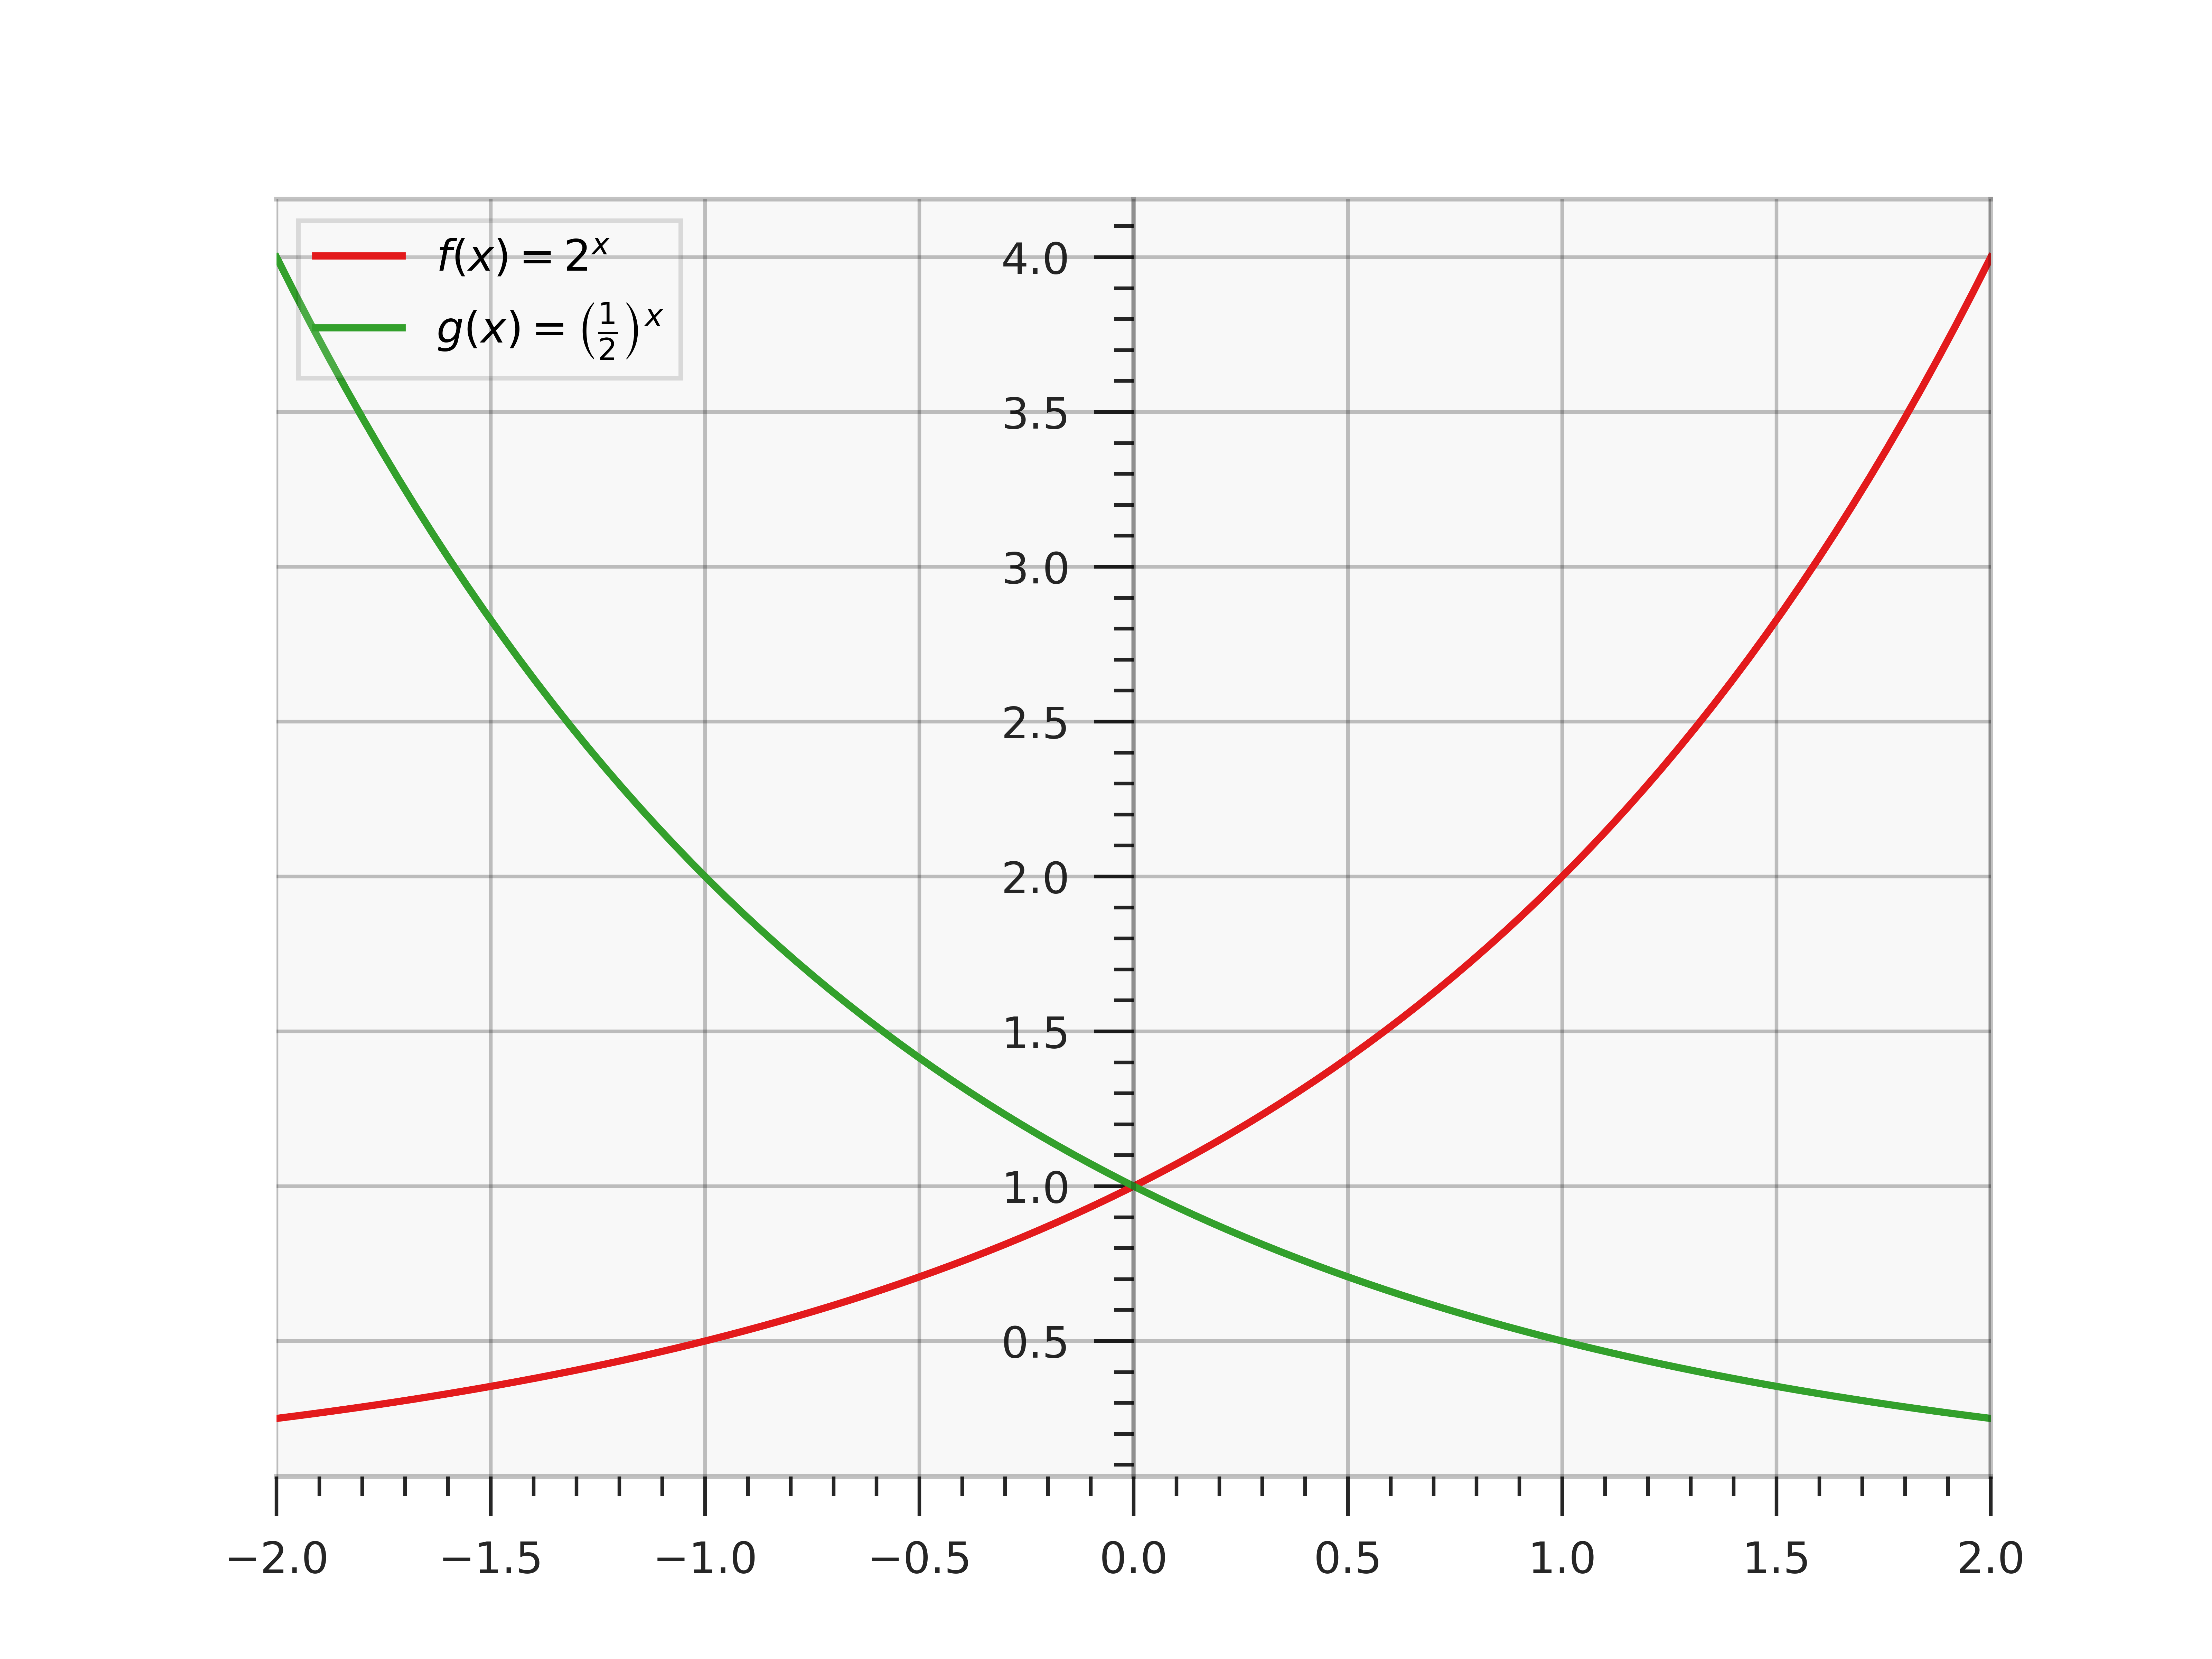
\includegraphics[width=12.5cm, height=10cm]{exponential_functions_1.png}
    \caption{Exponential Functions}
    \label{fig:fig1}
\end{figure}

The graph above highlights some useful properties of exponential functions.
Assuming the equations given above are satisfied, the properties of $f(x)=b^x$ are:

\begin{enumerate}
    \item $f(0) = 1 $. An exponential function will always be 1 at $x=0$.
    \item $f(x) \neq 0$. The function will never be equal to 0.
    \item $f(x) > 0$. The function will always be positive.
    \item The range of an exponential function is $(0, \infty)$.
    \item The domain of an exponential function is $(-\infty, \infty)$.
    \item If $0 < b < 1$, then:
          \begin{enumerate}
              \item $f(x) \rightarrow 0$ as $x \rightarrow \infty$
              \item $f(x) \rightarrow \infty$ as $x \rightarrow -\infty$
          \end{enumerate}
    \item If $b > 1$, then:
          \begin{enumerate}
              \item $f(x) \rightarrow \infty$ as $x \rightarrow \infty$
              \item $f(x) \rightarrow 0$ as $x \rightarrow -\infty$
          \end{enumerate}
\end{enumerate}

These are useful properties to remember throughout a Calculus course.
There is a special type of exponential function, where the base is euler's number, $e$.
This is called the natural exponential function, but is usually just referred to as the exponential function.

\begin{definition}
    The natural exponential function is:
    \begin{equation*}
        f(x) = e^x, e=2.71828182845905 \dots
    \end{equation*}
\end{definition}

As $e>0$, we know that $e^x \rightarrow \infty$ as $x \rightarrow \infty$ and $e^x \rightarrow 0$ as $x \rightarrow -\infty$.
Let's look at an example with this exponential function.

\begin{problem}
Sketch the graph of $h(t) = 1 - 5e^{1-\frac{t}{2}}$.
\end{problem}

Let's make a value table.

\begin{table}[H]
    \renewcommand{\arraystretch}{1.5}
    \centering
    \begin{tabular}{>{\centering\arraybackslash}m{1cm}|>{\centering\arraybackslash}m{2cm}}
        $t$  & $h(t)$     \\ \hline
        $-2$ & $-35.9453$ \\
        $-1$ & $-21.4084$ \\
        $0$  & $-12.5914$ \\
        $1$  & $	-7.2436$ \\
        $2$  & $	-4$
    \end{tabular}
\end{table}

We will sketch the above function in our chosen interval.

\begin{figure}[H]
    \centering
    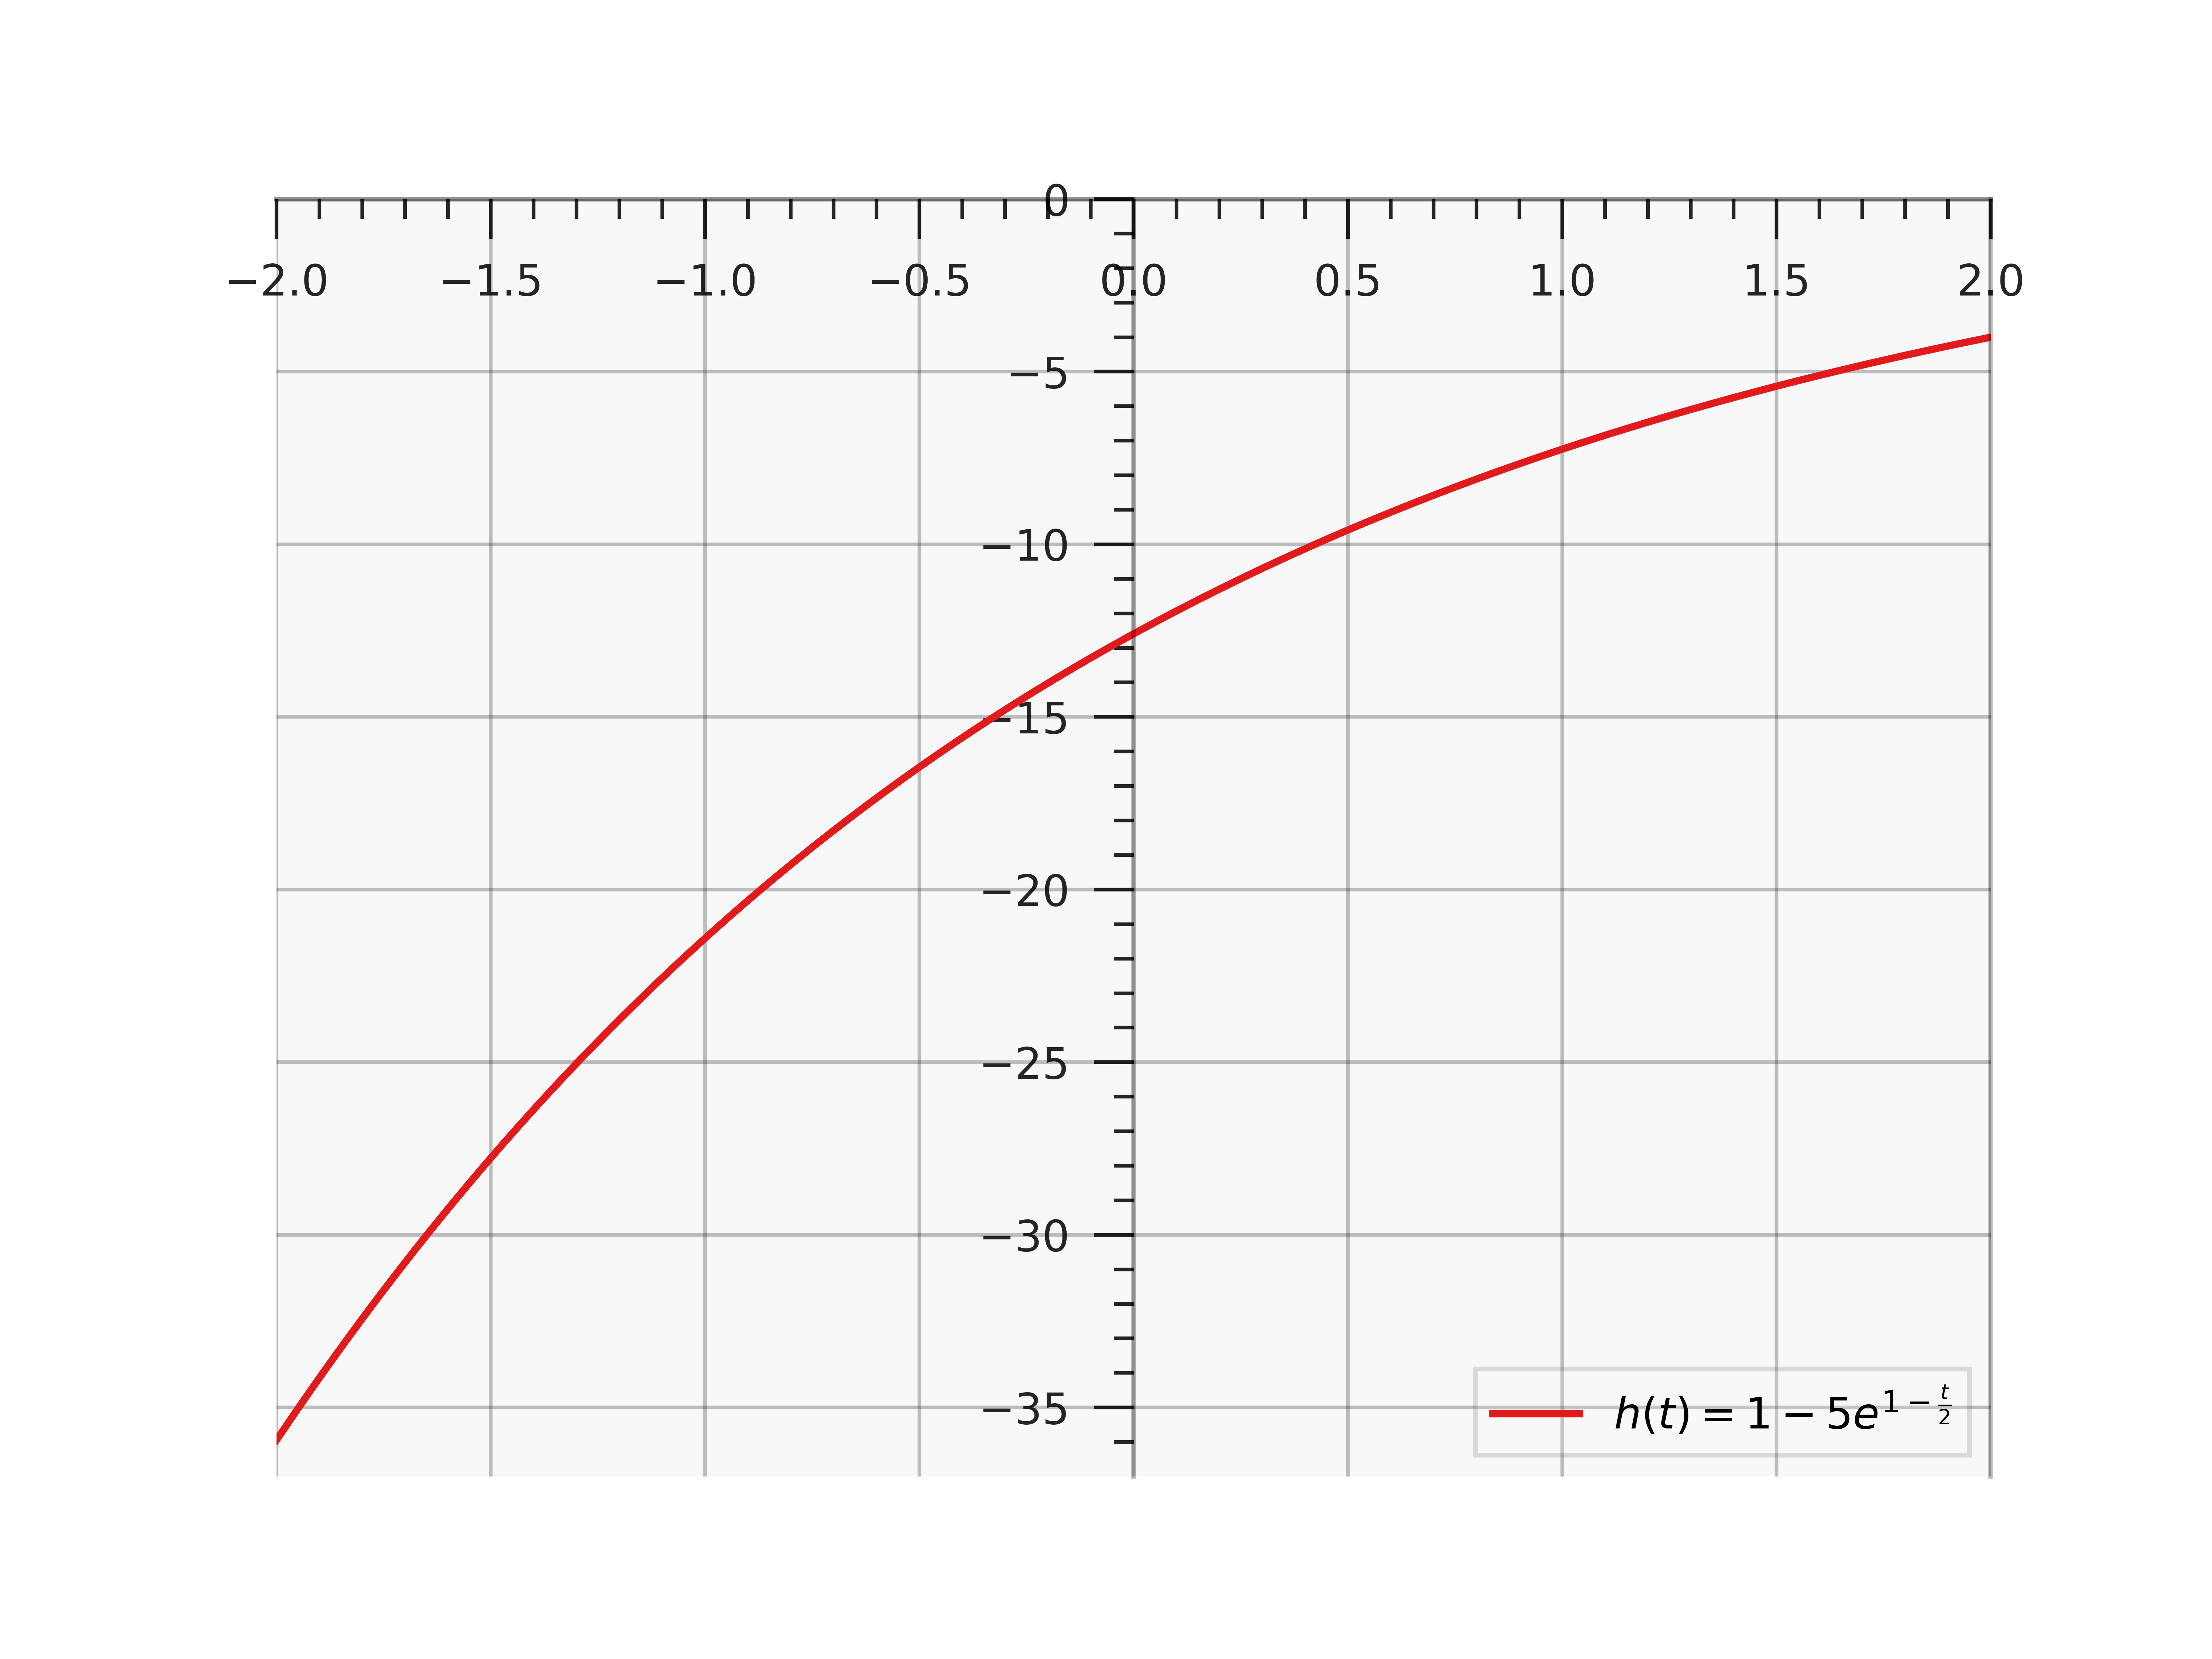
\includegraphics[width=12.5cm, height=10cm]{exponential_functions_2.png}
    \caption{Natural Exponential Functions}
    \label{fig:fig2}
\end{figure}

Being able to evaluate exponential functions is quite important.
Exponential functions will appear in most parts of Calculus I, particularly the natural exponential function.

\section{Logarithmic Functions}

Logarithmic functions are the opposite of exponential functions.
Considering some constant $b$ such that $b>0$ and $b\neq1$, it is true that $y=b^x$ is equivalent to $x=\log_b(y)$.
This equivalence is important to evaluate logarithms.

Let's evaluate some logarithms.

\begin{problem}
Without a calculator, give the exact values of the following:
\begin{enumerate}
    \item $\log_2(16)$
    \item $\log_4(16)$
    \item $\log_5(625)$
    \item $\log_9(\frac{1}{531441})$
    \item $\log_{\frac{1}{6}}(36)$
    \item $\log_{\frac{3}{2}}(\frac{27}{8})$
\end{enumerate}
\end{problem}

The easiest way to evaluate logarithms is usually to put them into exponential form.
For the first logarithm, we may say that it is equal to some number $x$.
Then, we would raise the number 2 by both sides of the equality, getting:

\begin{equation}
    2^x = 2^{\log_2(16)}
\end{equation}

As exponents and logarithms are inverses, raising some base by a logarithm of the same base effective cancel out.
Therefore, we have:

\begin{equation}
    2^x = 16
\end{equation}

Then it is obvious that our original logarithm evaluates to 4.
For the second logarithm, we may do the same thing (but with 4 as the base) and end up with:

\begin{equation}
    4^x = 16
\end{equation}

The second logarithm will thus evalaute to 2.
The third logarithm evaluates to 4 because $5^4=625$.
The fourth logarithm evalautes to $-6$ because $9^{-6}=\frac{1}{531441}$.
The fifth logarithm, while using a fractional base, can be evaluated in the same way.
We end up with the equation:

\begin{equation}
    \left(\frac{1}{6}\right)^x = 36
\end{equation}

We may simplify the left side to $6^{-x}$ to clearly see that the logarithm evaluates to $-2$.
The sixth logarithm evaluates to 3 because $\left(\frac{3}{2}\right)^3 = \frac{27}{8}$

There are some special logarithms that appear often in maths.
One of them is the common logarithm.
This is denoted by $log(x)$ and is equivalent to $log_10(x)$.
The other is the natural logarithm, written as $\ln(x)$.
This is equivelant to $\log_e(x)$, making the nautral logarithm the opposite of the exponential function $e^x$.
We will sketch them both below:

\begin{figure}[H]
    \centering
    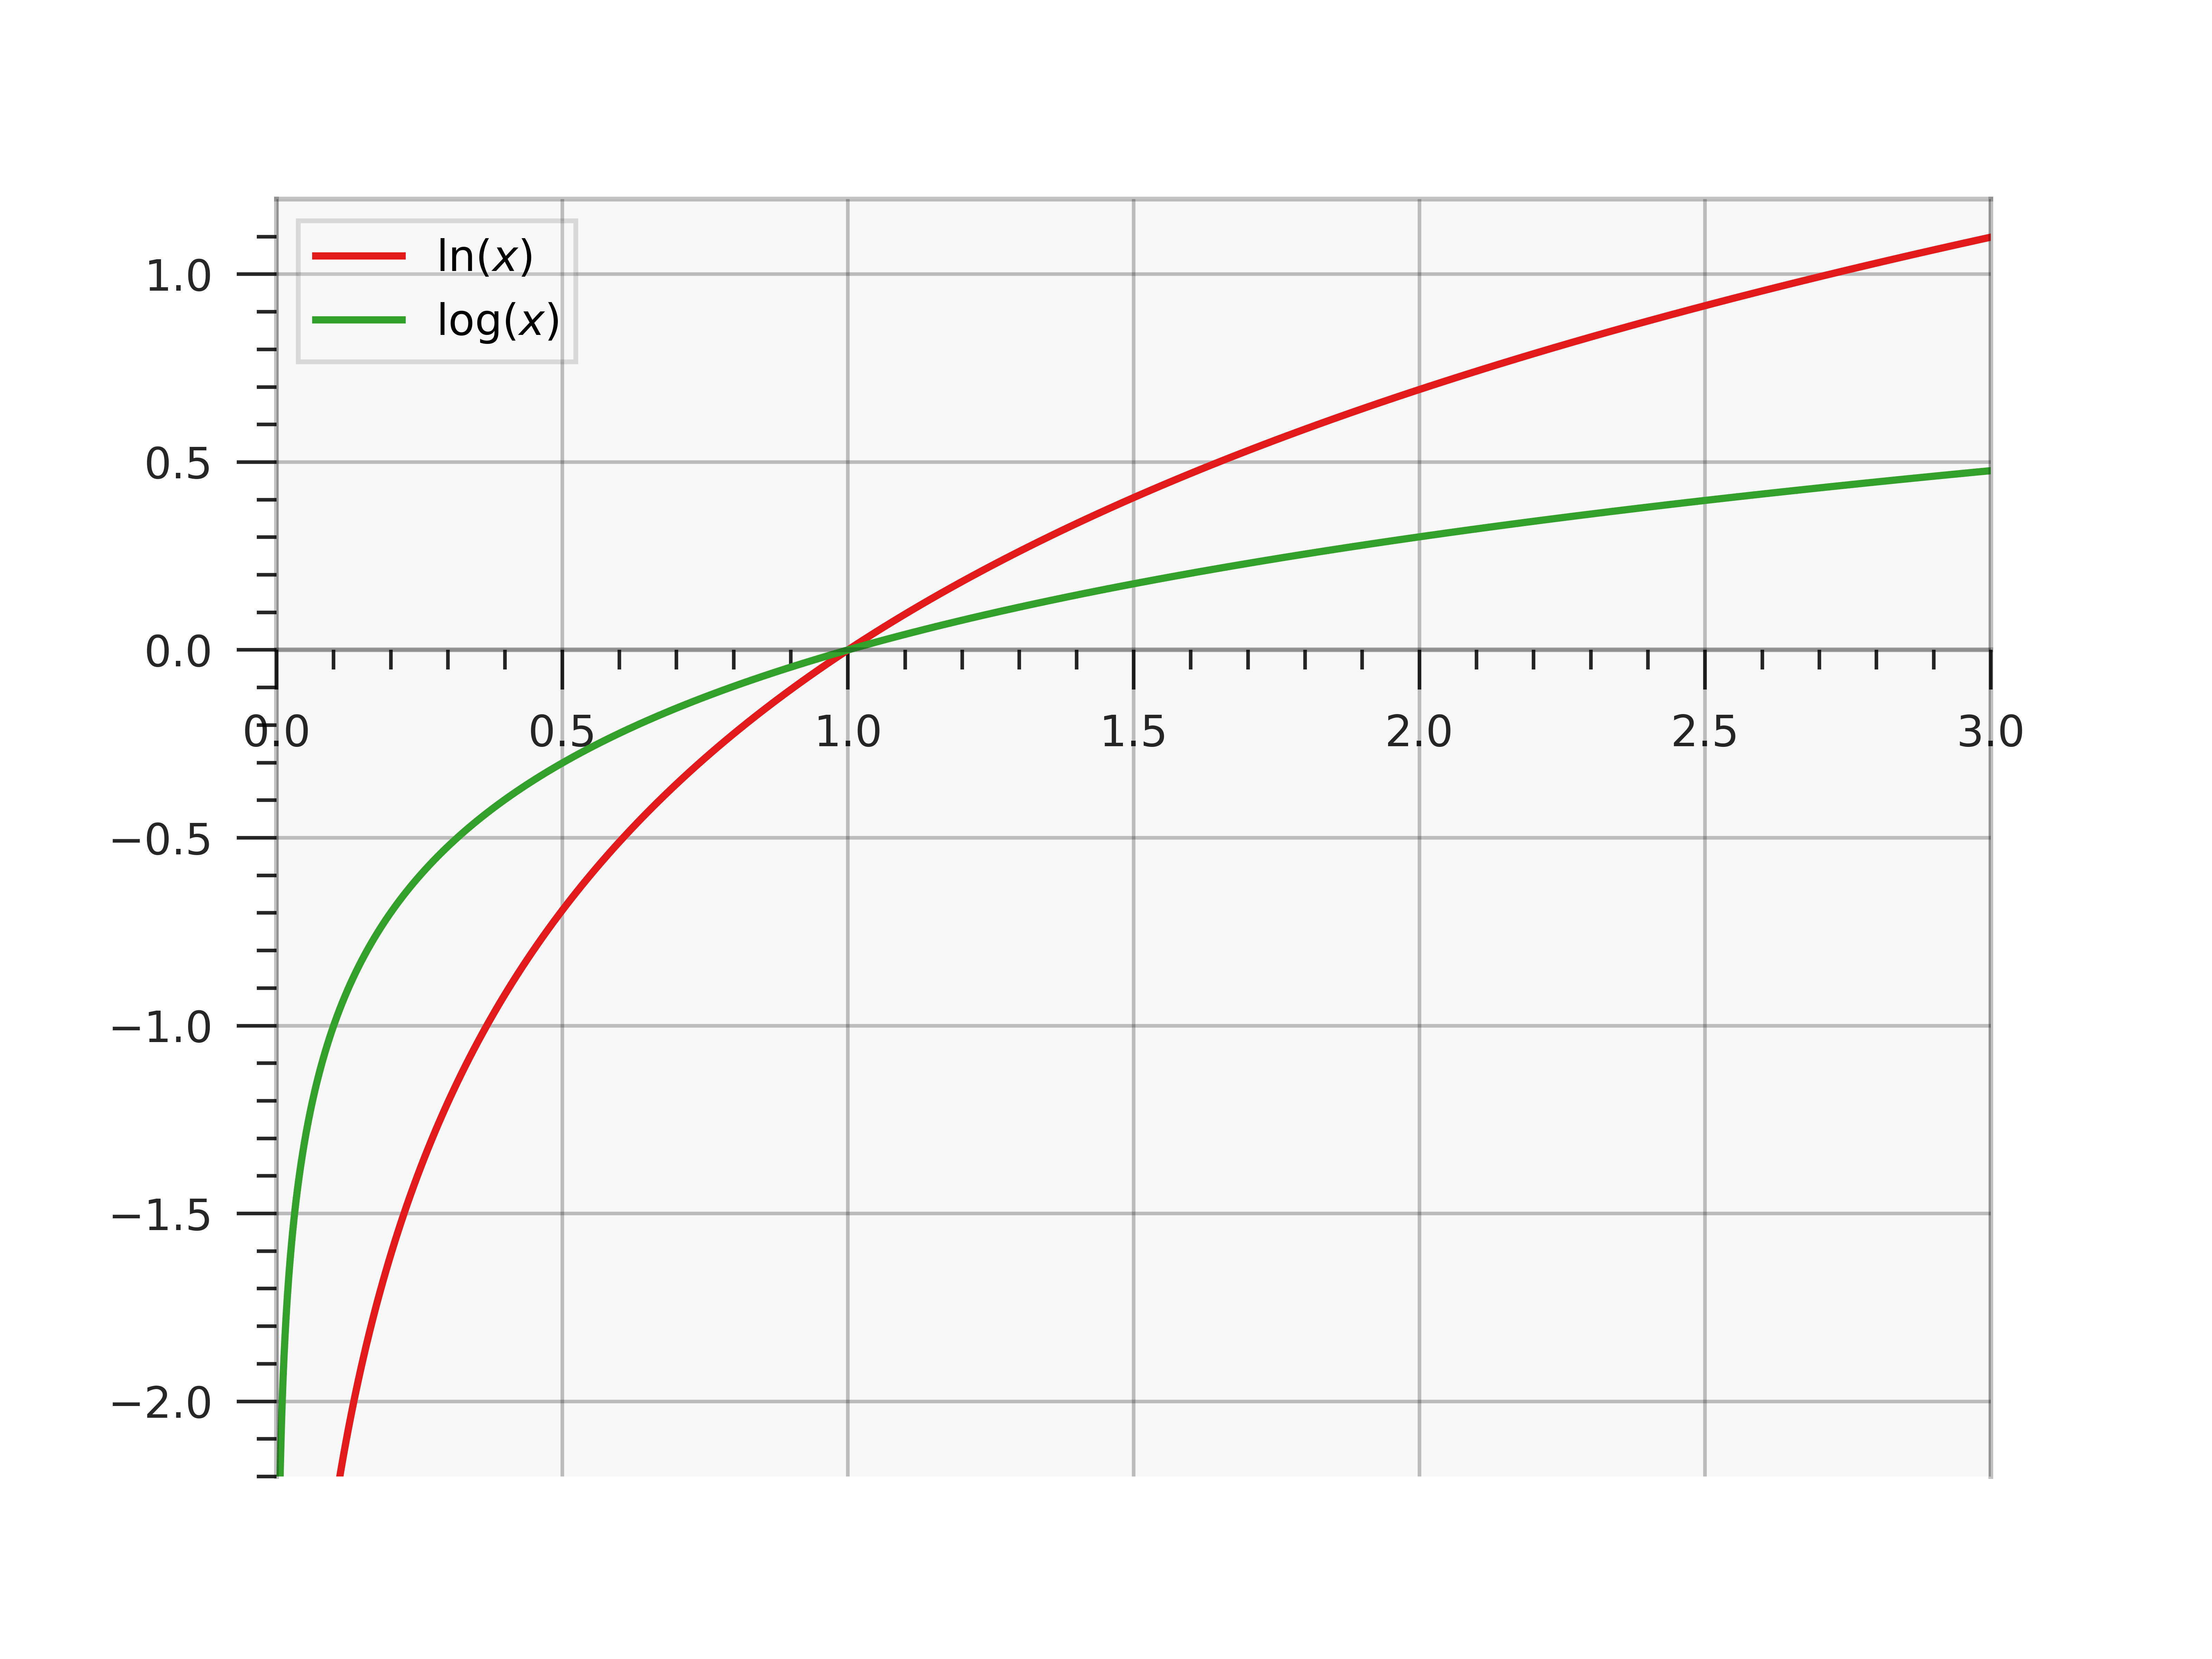
\includegraphics[width=12.5cm, height=10cm]{logarithmic_functions.png}
    \caption{Logarithmic Functions}
    \label{fig:fig3}
\end{figure}

The graph may be used to notice some useful properties of logarithmic functions that are often used in Calculus courses.
$\ln(x) \rightarrow \infty$ as $x \rightarrow \infty$.
Also, $\rightarrow -\infty$ as $x \rightarrow 0$, $x>0$.
It is important to note that the logairthm of 0 is undefined.

Let's evalaute some more logarithms.

\begin{problem}
Without a calculator, give the exact values of the following:
\begin{enumerate}
    \item $\ln(\sqrt[3]{e})$
    \item $\log(1000)$
    \item $\log_{16}(16)$
    \item $\log_{23}(1)$
    \item $\log_2(\sqrt[7]{32})$
\end{enumerate}
\end{problem}

For the first one, $\sqrt[3]{e}$ may be rewritten as $e^{\frac{1}{3}}$
As raising some base to a logarithm of the same base cancels out, the same is true for taking the logarithm with some base of that base raised to a power.
Then, taking the natural logarithm of $e$ raised to some number will return that number.
Therefore, the logarithm here will evaluate to $\frac{1}{3}$.

As $10^3=1000$, the second logarithm evaluates to 3.
When the number in the logarithm is the same as the base, the logairthm will obviously evaluate to 1 as any number raised by 1 will be the same number.
Therefore, the third logarithm evaluates to 1.
The logarithm of 1 with any base will be 0, as some number raised to the 0th power will be 1.
The fourth logarithm evaluates to 0.

For the last one, we may rewrite the logarithm as:

\begin{equation}
    2^x = \sqrt[7]{32}
\end{equation}

32 is also $2^5$ so $\sqrt[7]{32}$ is $\sqrt[7]{2^5}$.
With fractional exponents, this is $\left(2^5\right)^{\frac{1}{7}}$ or $2^\frac{5}{7}$.
It is then obvious the the logarithm evaluates to $\frac{5}{7}$.

We can write some general properties of logairthms.

\begin{enumerate}
    \item The domain of a logarithmic function is $(0, \infty)$. We cannot plug in negative numbers or 0.
    \item The range of a logarithmic function is $(-\infty, \infty)$.
    \item $\log_b(b)=1$
    \item $\log_b(1)=0$
    \item $\log_b(b^x)=x$
    \item $b^{\log_b(x)}=x$
\end{enumerate}

The last two properties show that exponential and logarithmic functions are inverses of each other.
If $f(x)=b^x$, then $f^{-1}(x)=\log_b(x)$.
There a couple more properties that allow for the manipulation of logarithmic expressions.

\begin{enumerate}
    \setcounter{enumi}{6}
    \item $\log_b(xy) = \log_b(x) + \log_b(y)$
    \item $\log_b\left(\frac{x}{y}\right) = \log_b(x) - \log_b(y)$
    \item $\log_b(x^y) = y\log_b(x)$
\end{enumerate}

Note that there is no property of logarithms that allows for the manipulation of sums and differences.
That means expressions like $\ln(x+y)$ and $\ln(x-y)$ are as simple as they can get.

We may use the above properties to simplify some logarithms.

\begin{problem}
Rewrite the following in terms of simpler logarithms:

\begin{enumerate}
    \item $\ln(x^3y^4z^5)$
    \item $\log_3\left(\frac{9x^4}{\sqrt{y}}\right)$
    \item $\log\left(\frac{x^2+y^2}{(x-y)^3}\right)$
\end{enumerate}
\end{problem}

We may simplify the first logarithm with property 7 and 9 as follows:

\begin{align}
     & \ln(x^3y^4z^5)                   \\
     & = \ln(x^3) + \ln(y^4) + \ln(z^5) \\
     & = 3\ln(x) + 4\ln(y) + 5\ln(z)
\end{align}

For the second logarithm, we will utilise properties 7, 8, and 9 as well as the fact that radicals may be represented with fractional exponents to simplify as follows:

\begin{align}
     & \log_3\left(\frac{9x^4}{\sqrt{y}}\right)          \\
     & = \log_3(9x^4) - \log_3(\sqrt{y})                 \\
     & = \log_3(9) + \log_3(x^4) - \log_3(y^\frac{1}{2}) \\
     & = 2 + 4\log_3(x) - \frac{1}{2} \log_3(y)
\end{align}

We may simplify the third logarithm with the same methods used above.

\begin{align}
     & \log\left(\frac{x^2+y^2}{(x-y)^3}\right) \\
     & = \log(x^2+y^2) - \log((x-y)^3)          \\
     & = \log(x^2+y^2) - 3\log(x-y)
\end{align}

We could apply property 9 on the second term as the whole term was raised to the third power.
The first term has a sum of terms that are individually squared so we cannot simplify it any further.

Now we will look at the change of base formula for logarithms.
The formula is:

\begin{equation}
    \log_b(x) = \frac{\log_a(x)}{\log_a(b)}
\end{equation}

This is the general formula to convert from some base $b$ to $a$.
However, the change of base formula is usually used to calculate the value of logarithms that are in base which is difficult to deal with.
The two most common formulae are:

\begin{equation}
    \log_b(x) = \frac{\ln(x)}{\ln(b)} \qquad~\qquad \log_b(x) = \frac{\log(x)}{\log(b)}
\end{equation}

Either of the above may be listed as the change of base formula.
The formula is usually used with calculators that only have buttons for the common and natural logarithm.
Otherwise, there is not much use to the formula when evalauting logairthms with a calculator.

The logarithms evaluated above could be done easily because they could be written in terms of a base to some power.
For instance, $\log_7(49)=2$ because $7^2=49$.
However, evalauting $\log_7(50)$ is more difficult and would require using a change of base formula to evaluate on a calculator that doesn't allow for logarithms with any base.

\begin{equation}
    \log_7(50) = \frac{\ln(50)}{\ln(7)} = \frac{3.91202300543}{1.94591014906} = 2.0103821378
\end{equation}

or

\begin{equation}
    \log_7(50) = \frac{\log(50)}{\log(7)} = \frac{1.69897000434}{0.845098040014} = 2.0103821378
\end{equation}

We could do this for any logarithm but ones that can be evaluated simply such as $\log_7(49)$ would take more effort than evaluating normally.

We have covered how logarithms work and some properties which allow for the manipulation of logarithmic expressions.
While they do not appear as often as exponential functions, they still do appear on occasion in Calculus courses.

\end{document}